% ==============================================================================
% CAPÍTULO 3: METODOLOGIA
%
% EQUAÇÕES NESTE CAPÍTULO: as que OPERACIONALIZAM a pesquisa ("como este
% estudo mede, estima, compara ou decide"): métricas de avaliação, modelo a
% ser estimado, transformações dos dados, critérios de seleção. Equações já
% definidas na Fundamentação teórica NÃO são repetidas: basta \eqref e as
% decisões operacionais. Equações com valores estimados (coeficientes
% obtidos) são achados e vão para os Resultados. Ver exemplos na Seção 3.6.
% ==============================================================================
\chapter{Metodologia}
\label{ch:metodologia}
\begin{resumocapitulo}
  Aqui deve ser incluído um resumo do capítulo, descrevendo, de forma reduzida, os procedimentos metodológicos empregados para operacionalizar a investigação e responder aos objetivos propostos na pesquisa. Apresenta-se o delineamento epistemológico do estudo, detalhando a natureza da abordagem, a classificação tipológica e as etapas sistemáticas do processo investigativo. São especificados o universo amostral, os critérios de seleção e extração de dados e as ferramentas técnicas utilizadas na coleta das informações.
\end{resumocapitulo}

\preencher{A metodologia tem como finalidade descrever e justificar o percurso sistemático adotado para responder ao problema de pesquisa e atingir os objetivos propostos. Seu papel estrutural é detalhar os pressupostos epistemológicos, a classificação do estudo, os procedimentos de coleta, os critérios de amostragem e as técnicas de análise e validação dos dados. Ela confere rigor científico, reprodutibilidade e transparência à investigação, assegurando a validade interna e externa dos resultados obtidos. Apagar esse texto de instrução após a redação da seção.}

\section{Visão geral}
\label{sec:visao_geral_metodologia}
Descrever uma síntese do que será tratado no capítulo, incluindo a natureza da pesquisa, a abordagem metodológica, os objetivos específicos e os procedimentos técnicos adotados. A visão geral deve fornecer ao leitor um panorama do desenho investigativo, destacando como cada etapa contribui para responder à pergunta de pesquisa e alcançar os objetivos propostos.

\section{Classificação da pesquisa}
\label{sec:classificacao}
A classificação da pesquisa tem como finalidade enquadrar o estudo quanto à sua natureza (básica ou aplicada), à abordagem do problema (quantitativa, qualitativa ou mista), aos objetivos (exploratória, descritiva ou explicativa) e aos procedimentos técnicos (bibliográfica, documental, experimental, levantamento, estudo de caso, entre outros). Cada enquadramento precisa ser justificado com apoio na literatura metodológica, e não apenas declarado.

\section{Desenho da pesquisa}
\label{sec:desenho_pesquisa}
O desenho da pesquisa tem como finalidade estabelecer a arquitetura lógica e o plano conceitual da investigação, integrando a estratégia metodológica aos objetivos do estudo. O seu papel estrutural é explicitar o encadeamento causal e operacional entre os dados, as hipóteses ou questões norteadoras e as técnicas de inferência aplicadas. Ele fornece a visão panorâmica do percurso investigativo e demonstra que os procedimentos adotados constituem um sistema coeso, capaz de sustentar empiricamente as conclusões da dissertação. Recomenda-se representar esse percurso em uma figura que associe cada etapa ao objetivo específico correspondente.

\section{Procedimentos de levantamento da literatura}
\label{sec:procedimentos_literatura}
Os procedimentos de levantamento da literatura têm como finalidade formalizar o protocolo técnico e auditável adotado para a recuperação das fontes científicas. O seu papel estrutural é detalhar as bases de dados bibliográficas consultadas, os termos de busca e operadores booleanos aplicados, o horizonte temporal, as regras de filtragem e os critérios objetivos de inclusão e exclusão. Esse detalhamento garante a reprodutibilidade da triagem, reduz o viés de seleção manual e fundamenta a integridade epistemológica do estado da arte discutido no Capítulo~\ref{ch:fundamentacao_teorica}. O fluxo de seleção é apresentado na Figura~\ref{fig:diagrama_prisma}, e as \textit{strings} de busca aplicadas em cada base encontram-se no Apêndice~\ref{ap:ap_string}.

\begin{figure}[H]
  \centering
  \caption{Fluxograma do processo de seleção sistemática conforme a recomendação PRISMA 2020}
  % ==============================================================================
% Fluxograma PRISMA 2020 (Page et al., 2021): identificação por bases de dados
% e registros. Preencher os valores de n. Incluído por \input no Capítulo 3.
% ==============================================================================
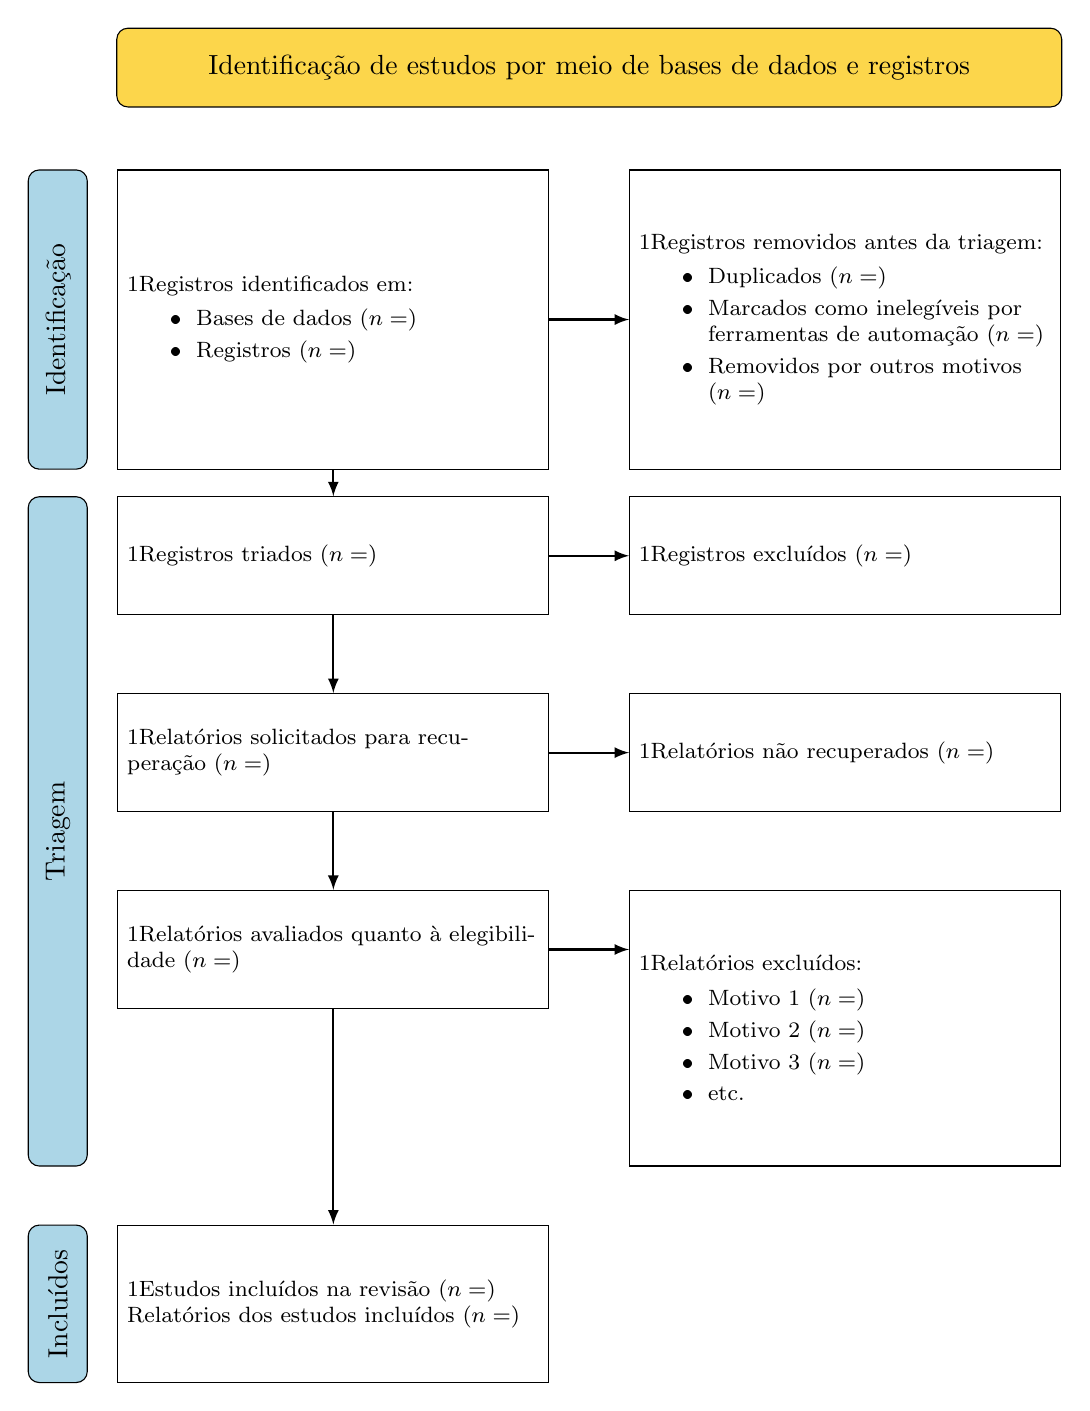
\begin{tikzpicture}[>=latex, font={\sffamily\small}]

    \tikzset{
      bluerect/.style={rectangle, rounded corners, minimum width=1.5cm, minimum height=0.75cm,
                       text centered, draw=black, fill=cyan!60!gray!45!white, rotate=90, font=\rmfamily},
      roundedrect/.style={rectangle, rounded corners, minimum width=12cm, minimum height=1cm,
                          text centered, draw=black, font=\rmfamily},
      textrect/.style={rectangle, minimum width=5.25cm, text width=5.24cm, minimum height=1cm,
                       draw=black, font={\rmfamily\footnotesize},
                       execute at begin node={\setstretch{1}\setlength{\itemsep}{0pt}}}
    }

    \node (top1) at (0, 11.2cm) [roundedrect, fill=yellow!80!red!70]
    {Identificação de estudos por meio de bases de dados e registros};

    \node (r1blue) at (-6.75cm, 8.0cm) [bluerect, minimum width=3.8cm]{Identificação};

    \node (r1left) at (-3.25cm, 8.0cm) [textrect, minimum height=3.8cm]
    {Registros identificados em:
        \begin{itemize}\setlength{\itemsep}{0pt}\setlength{\parsep}{0pt}\setlength{\topsep}{2pt}
            \item Bases de dados ($n=$)
            \item Registros ($n=$)
        \end{itemize}
    };

    \node (r1right) at (3.25cm, 8.0cm) [textrect, minimum height=3.8cm]
    {Registros removidos antes da triagem:
        \begin{itemize}\setlength{\itemsep}{0pt}\setlength{\parsep}{0pt}\setlength{\topsep}{2pt}
            \item Duplicados ($n=$)
            \item Marcados como inelegíveis por ferramentas de automação ($n=$)
            \item Removidos por outros motivos ($n=$)
        \end{itemize}
    };

    \node (r2blue) at (-6.75cm, 1.5cm) [bluerect, minimum width=8.5cm]{Triagem};

    \node (r2left) at (-3.25cm, 5.0cm) [textrect, minimum height=1.5cm]
    {Registros triados ($n=$)};

    \node (r2right) at (3.25cm, 5.0cm) [textrect, minimum height=1.5cm]
    {Registros excluídos ($n=$)};

    \node (r3left) at (-3.25cm, 2.5cm) [textrect, minimum height=1.5cm]
    {Relatórios solicitados para recuperação ($n=$)};

    \node (r3right) at (3.25cm, 2.5cm) [textrect, minimum height=1.5cm]
    {Relatórios não recuperados ($n=$)};

    \node (r4left) at (-3.25cm, 0cm) [textrect, minimum height=1.5cm]
    {Relatórios avaliados quanto à elegibilidade ($n=$)};

    \node (r4right) at (3.25cm, -1.0cm) [textrect, minimum height=3.5cm]
    {Relatórios excluídos:
        \begin{itemize}\setlength{\itemsep}{0pt}\setlength{\parsep}{0pt}\setlength{\topsep}{2pt}
            \item Motivo 1 ($n=$)
            \item Motivo 2 ($n=$)
            \item Motivo 3 ($n=$)
            \item etc.
        \end{itemize}
    };

    \node (r5blue) at (-6.75cm, -4.5cm) [bluerect, minimum width=2cm]{Incluídos};

    \node (r5left) at (-3.25cm, -4.5cm) [textrect, minimum height=2cm]
    {Estudos incluídos na revisão ($n=$)\\
     Relatórios dos estudos incluídos ($n=$)};

    % Conectores
    \draw[thick, ->] (r1left) -- (r1right);
    \draw[thick, ->] (r1left) -- (r2left);
    \draw[thick, ->] (r2left) -- (r2right);
    \draw[thick, ->] (r2left) -- (r3left);
    \draw[thick, ->] (r3left) -- (r3right);
    \draw[thick, ->] (r3left) -- (r4left);
    % Corrigido: no original, "-+ (0.5,0)" não alcançava a caixa de excluídos
    \draw[thick, ->] (r4left.east) -- (r4left.east -| r4right.west);
    \draw[thick, ->] (r4left) -- (r5left);

\end{tikzpicture}
 % apenas o código TikZ, sem o ambiente figure
  \label{fig:diagrama_prisma}
  \fonte{Elaborada pelo autor (\ano).}
\end{figure}

\section{Procedimentos de coleta de dados}
\label{sec:coleta}
Esta seção tem como finalidade caracterizar a origem empírica da pesquisa: o universo e a amostra (ou as bases e repositórios utilizados), os critérios de seleção, os instrumentos de coleta (questionários, roteiros de entrevista, \textit{datasets}, APIs) e o período de realização. Quando houver instrumento próprio, convém descrever sua construção, as escalas adotadas e os procedimentos de pré-teste ou validação de conteúdo.

\section{Procedimentos de análise de dados}
\label{sec:analise}
Os procedimentos de análise têm como finalidade descrever as técnicas estatísticas, computacionais ou interpretativas aplicadas aos dados, os critérios de avaliação adotados e as ferramentas utilizadas (linguagens, bibliotecas e versões). Cada técnica deve estar vinculada ao objetivo específico que pretende atender. É também aqui que se definem os critérios de validação dos resultados, tais como métricas de desempenho, testes de robustez, confiabilidade de escalas ou triangulação de fontes.

% ------------------------------------------------------------------------------
% EXEMPLOS DE EXPRESSÕES MATEMÁTICAS (adaptar ou apagar)
% Regras gerais (NBR 14724:2024):
% - Expressões curtas podem ficar no próprio parágrafo, entre $...$.
% - Equações destacadas ficam centralizadas e numeradas à direita, entre
%   parênteses; a classe numera por capítulo: (3.1), (3.2)...
% - Toda equação destacada deve ser citada no texto com \eqref{rótulo}, que
%   gera o número com os parênteses: Equação~\eqref{eq:f1}.
% - A equação faz parte da frase: termina com vírgula ou ponto, e as
%   variáveis são definidas logo após, com "em que" ou "onde".
% - Notação, letras e símbolos devem ser os mesmos em todo o trabalho;
%   havendo muitos, registrá-los na Lista de símbolos.
% - Cada equação aparece UMA vez no trabalho, no capítulo de sua função
%   principal; nos demais, é retomada por \eqref.
% ------------------------------------------------------------------------------
\begin{orientacao}[Equações na metodologia]
  Nesta seção entram as expressões que operacionalizam a pesquisa, isto é, as que mostram \emph{como este estudo} mede, estima, compara ou decide: métricas de avaliação, especificação do modelo a ser estimado, transformações aplicadas aos dados e critérios de seleção. Equações já definidas na Fundamentação teórica não devem ser repetidas; basta remeter a elas e descrever as decisões operacionais (algoritmo, parâmetros, amostra, biblioteca e versão), como no primeiro parágrafo de exemplo abaixo. Equações com valores estimados, como um modelo ajustado com seus coeficientes, são achados da pesquisa e pertencem aos Resultados (Capítulo~\ref{ch:analise_discussao}).
\end{orientacao}

% Exemplo 0: remissão a uma equação da Fundamentação teórica
% A definição (Equação 2.1) NÃO é repetida. Esta seção acrescenta apenas
% o que o estudo decidiu: algoritmo, biblioteca, versão e amostra.
A contribuição de cada variável preditora para as predições foi estimada pelos valores de Shapley, definidos na Equação~\eqref{eq:shapley} (Seção~\ref{sec:construto_1}). Como o cálculo exato exige avaliar $2^{|N|-1}$ coalizões para cada variável, o que o torna inviável quando há muitas variáveis, adotou-se o algoritmo TreeSHAP \cite{Lundberg2020}, que obtém os valores exatos em tempo polinomial para modelos baseados em árvores de decisão. Os cálculos foram realizados com a biblioteca \textit{shap}, versão \preencher{x.y.z}, sobre uma amostra de referência de \preencher{n} observações.

% Exemplo 1: expressão no corpo do texto (definições operacionais do estudo)
O desempenho dos classificadores foi avaliado a partir da matriz de confusão, cujos elementos são os verdadeiros positivos ($VP$), os falsos positivos ($FP$) e os falsos negativos ($FN$). Considerou-se como limiar de decisão o valor $\tau = 0{,}5$, aplicado à probabilidade estimada $\hat{p}_i \in [0, 1]$ de cada observação $i$.

% Exemplo 2: conjunto de equações alinhadas pelo sinal de igualdade
% (ambiente align; cada linha recebe seu próprio número e rótulo)
A precisão e a revocação foram calculadas conforme as Equações~\eqref{eq:precisao} e~\eqref{eq:revocacao}:
\begin{align}
  \text{Precisão}  & = \frac{VP}{VP + FP}, \label{eq:precisao}  \\
  \text{Revocação} & = \frac{VP}{VP + FN}. \label{eq:revocacao}
\end{align}

% Exemplo 3: equação destacada, seguida da definição das variáveis
% (métrica escolhida pelo pesquisador como critério de avaliação: por
% isso está na Metodologia, e não na Fundamentação)
Como as classes são desbalanceadas, adotou-se como métrica principal o \textit{F1-score}, média harmônica entre precisão e revocação, expressa na Equação~\eqref{eq:f1}:
\begin{equation}
  F_1 = 2 \cdot \frac{\text{Precisão} \cdot \text{Revocação}}{\text{Precisão} + \text{Revocação}},
  \label{eq:f1}
\end{equation}
em que $F_1 \in [0, 1]$, sendo 1 o desempenho máximo.

% Exemplo 4: problema de otimização (\argmin está definido na classe)
Os hiperparâmetros $\theta$ de cada modelo foram ajustados por validação cruzada com $k$ partições, minimizando a perda média, conforme a Equação~\eqref{eq:otimizacao}:
\begin{equation}
  \hat{\theta} = \argmin_{\theta \in \Theta} \; \frac{1}{k} \sum_{m=1}^{k} \mathcal{L}\left(\theta;\, D_m\right),
  \label{eq:otimizacao}
\end{equation}
onde $\Theta$ é o espaço de busca dos hiperparâmetros, $D_m$ é a $m$-ésima partição de validação e $\mathcal{L}$ é a função de perda.

% ------------------------------------------------------------------------------
% EXEMPLO DE PSEUDOCÓDIGO (adaptar ou apagar)
% Pacote algorithm2e, já carregado pela classe com as opções: português,
% moldura "ruled", linhas verticais de bloco e linhas numeradas.
% Regras gerais:
% - O pseudocódigo descreve o PROCEDIMENTO, de forma independente da
%   linguagem de programação. O código-fonte efetivo vai para um Apêndice.
% - Título ACIMA (\caption) e \label logo depois; citar no texto ANTES, com
%   Algoritmo~\ref{rótulo}.
% - Declarar entradas (\KwIn) e saídas (\KwOut) e usar a MESMA notação das
%   equações do texto (aqui: \theta, \Theta, k, D_m e \mathcal{L}).
% - Uma instrução por linha, terminada com \; . Comentários com \tcp{...}.
% - Blocos: \ForEach{...}{...}, \For{...}{...}, \If{...}{...}, \eIf{...}{...}{...},
%   \While{...}{...}; atribuição com \leftarrow; retorno com \Return.
% - Funções nomeadas: \SetKwFunction{\Nome}{nome} e \Nome{argumentos}.
% - Havendo vários algoritmos, incluir \listofalgorithms em
%   pre-textuais/listas.tex (Lista de algoritmos, opcional).
% - Fonte: os algoritmos não exigem \fonte, mas, se adaptados de outro
%   trabalho, a origem deve ser citada no texto.
% ------------------------------------------------------------------------------
\begin{orientacao}[Pseudocódigo na metodologia]
  O pseudocódigo descreve um procedimento de forma precisa e independente da linguagem de programação, permitindo que outro pesquisador o reproduza. Ele complementa a equação: enquanto a Equação~\eqref{eq:otimizacao} define \emph{o que} é otimizado, o Algoritmo~\ref{alg:selecao_hiperparametros} mostra \emph{como} a busca é executada. Use a mesma notação das equações e reserve o código-fonte efetivo para um Apêndice.
\end{orientacao}

% Exemplo 5: pseudocódigo do procedimento definido na Equação 3.4
A busca pelos hiperparâmetros que minimizam a Equação~\eqref{eq:otimizacao} foi realizada por busca em grade, conforme o procedimento descrito no Algoritmo~\ref{alg:selecao_hiperparametros}. Para cada combinação candidata $\theta \in \Theta$, o modelo é treinado em $k-1$ partições e avaliado na partição restante, e a combinação com menor perda média é selecionada.

\begin{algorithm}[H]
  \caption{Seleção de hiperparâmetros por busca em grade com validação cruzada}
  \label{alg:selecao_hiperparametros}
  \SetKwFunction{Treinar}{treinar}
  \SetKwFunction{Perda}{perda}
  \KwIn{conjunto de treinamento $D$; espaço de busca $\Theta$; número de partições $k$}
  \KwOut{hiperparâmetros selecionados $\hat{\theta}$}
  dividir $D$ em $k$ partições estratificadas $D_1, \dots, D_k$\;
  $\hat{\theta} \leftarrow$ nulo; \quad $L^{*} \leftarrow +\infty$\;
  \ForEach{$\theta \in \Theta$}{
    $S \leftarrow 0$ \tcp*{soma das perdas nas partições}
    \For{$m \leftarrow 1$ \KwTo $k$}{
      $f \leftarrow$ \Treinar{$D \setminus D_m$, $\theta$}\;
      $S \leftarrow S + $ \Perda{$f$, $D_m$}\;
    }
    \If(\tcp*[f]{perda média menor que a melhor até aqui}){$S/k < L^{*}$}{
      $L^{*} \leftarrow S/k$\;
      $\hat{\theta} \leftarrow \theta$\;
    }
  }
  \Return{$\hat{\theta}$}\;
\end{algorithm}

Ao final, o modelo é treinado novamente com $\hat{\theta}$ sobre todo o conjunto de treinamento, e só então avaliado no conjunto de teste, que não participa do Algoritmo~\ref{alg:selecao_hiperparametros}.

% ------------------------------------------------------------------------------
% EXEMPLOS DE FIGURAS (adaptar ou apagar)
% Regras gerais (NBR 14724:2024):
% - A identificação (palavra Figura, número e título) fica ACIMA da imagem,
%   com \caption antes de \includegraphics; a fonte fica ABAIXO, com \fonte.
% - O \label vem DEPOIS do \caption (caso contrário, a referência aponta
%   para o número errado).
% - Toda figura deve ser citada no texto ANTES de aparecer, com
%   Figura~\ref{rótulo}; o til impede a quebra de linha entre palavra e número.
% - Arquivos ficam na pasta figuras/. Prefira PDF (vetorial) para gráficos
%   gerados por código; para imagens raster (PNG/JPG), use no mínimo 300 dpi.
%   A extensão pode ser omitida: \includegraphics{figuras/arquivo}.
% - Dimensione pela largura do texto (\textwidth) ou da coluna (\linewidth),
%   nunca em centímetros fixos, para preservar a proporção.
% - Figura elaborada pelo próprio autor: "Elaborada pelo autor (\ano)".
%   Figura reproduzida ou adaptada: "Adaptada de \citeonline{Chave}".
% ------------------------------------------------------------------------------
\begin{orientacao}[Figuras na metodologia]
  Os exemplos a seguir ilustram duas formas de inserir imagens: figuras isoladas, cada uma ocupando a largura útil do texto, e figuras dispostas lado a lado, recurso indicado quando o leitor precisa comparar dois elementos visuais relacionados. Os valores representados são fictícios. No trabalho real, figuras que exibem valores efetivamente obtidos (contagens da matriz de confusão, desempenho dos modelos) constituem achados da pesquisa e pertencem aos Resultados (Capítulo~\ref{ch:analise_discussao}); na Metodologia, cabem figuras que descrevem procedimentos, como fluxos, arquiteturas e esquemas de validação. Cada figura deve aparecer uma única vez no trabalho; os exemplos lado a lado repetem as mesmas imagens apenas para fins didáticos.
\end{orientacao}

% Exemplo 6: figuras isoladas (um ambiente figure para cada imagem)
A Figura~\ref{fig:matriz_confusao} apresenta a matriz de confusão do classificador de melhor desempenho, com os elementos $VP$, $FP$, $FN$ e $VN$ obtidos para o limiar $\tau = 0{,}5$.

\begin{figure}[H]
  \centering
  \caption{Matriz de confusão do classificador XGBoost no conjunto de teste}
  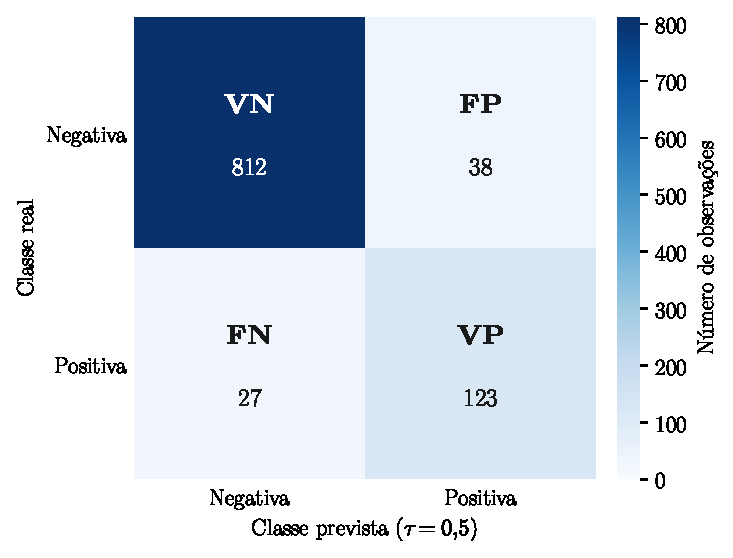
\includegraphics[width=0.65\textwidth]{figuras/matriz_confusao}
  \label{fig:matriz_confusao}
  \fonte{Elaborada pelo autor (\ano).}
\end{figure}

A Figura~\ref{fig:f1_classificadores} compara o \textit{F1-score} (Equação~\eqref{eq:f1}) dos quatro classificadores avaliados nas $k = 5$ partições da validação cruzada. As barras indicam a média, as hastes o desvio-padrão e os pontos o valor obtido em cada partição.

\begin{figure}[H]
  \centering
  \caption{Desempenho dos classificadores segundo o \textit{F1-score} na validação cruzada}
  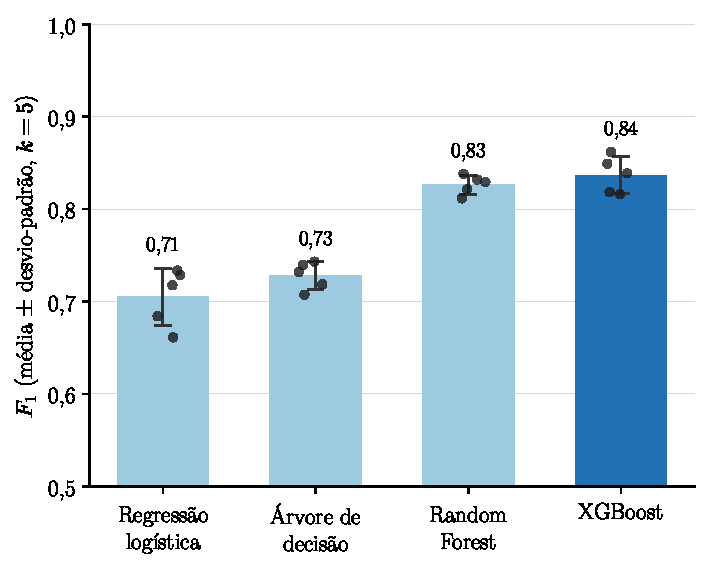
\includegraphics[width=0.75\textwidth]{figuras/f1_classificadores}
  \label{fig:f1_classificadores}
  \fonte{Elaborada pelo autor (\ano).}
\end{figure}

% Exemplo 7: figuras lado a lado (dois minipage dentro de um único figure)
% Cada minipage recebe seu próprio \caption, \label e \fonte, e cada imagem
% é numerada como uma figura independente. A soma das larguras (0.48 + 0.48)
% deve ficar abaixo de 1\textwidth; o \hfill distribui o espaço restante.
% Não deixe linha em branco entre os minipage, ou eles serão empilhados.
% A mesma altura máxima (height + keepaspectratio) nas duas imagens alinha
% as fontes na mesma linha, mesmo com proporções diferentes.
As Figuras~\ref{fig:matriz_confusao_lado} e~\ref{fig:f1_classificadores_lado} apresentam, lado a lado, a matriz de confusão e o desempenho comparativo dos classificadores, o que permite relacionar a distribuição dos erros do melhor modelo à sua posição relativa entre as alternativas avaliadas.

\begin{figure}[H]
  \centering
  \begin{minipage}[t]{0.48\textwidth}
    \centering
    \caption{Matriz de confusão do classificador XGBoost}
    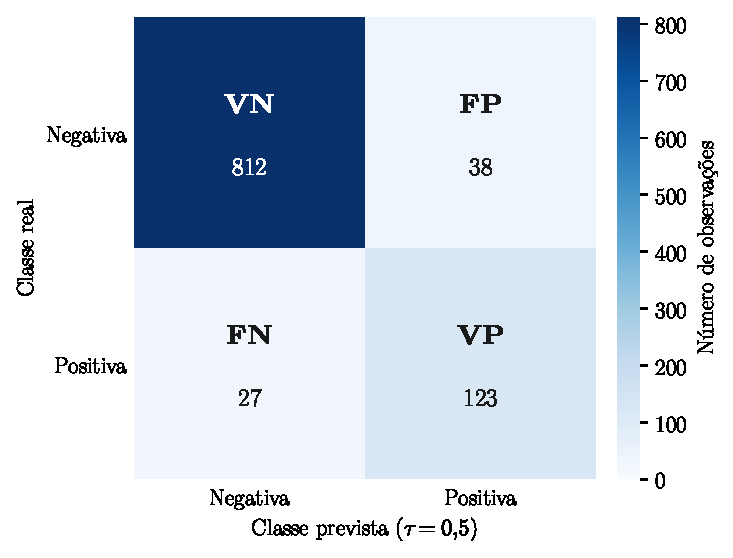
\includegraphics[width=\linewidth,height=0.74\linewidth,keepaspectratio]{figuras/matriz_confusao}
    \label{fig:matriz_confusao_lado}
    \fonte{Elaborada pelo autor (\ano).}
  \end{minipage}%
  \hfill
  \begin{minipage}[t]{0.48\textwidth}
    \centering
    \caption{\textit{F1-score} dos classificadores na validação cruzada}
    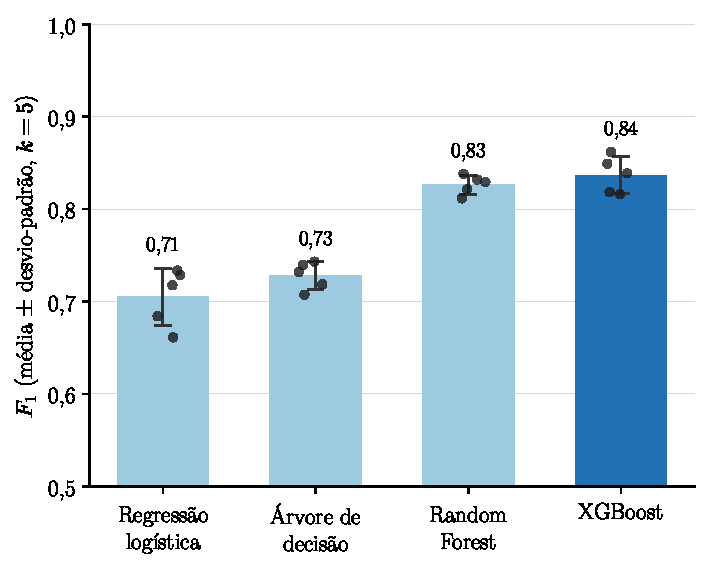
\includegraphics[width=\linewidth,height=0.74\linewidth,keepaspectratio]{figuras/f1_classificadores}
    \label{fig:f1_classificadores_lado}
    \fonte{Elaborada pelo autor (\ano).}
  \end{minipage}
\end{figure}

\section{Aspectos éticos}
\label{sec:aspectos_eticos}
Pesquisas que envolvem seres humanos, direta ou indiretamente (questionários, entrevistas, dados pessoais), devem ser submetidas ao Comitê de Ética em Pesquisa por meio da Plataforma Brasil, em conformidade com as Resoluções CNS n.º 466/2012 e n.º 510/2016. Nesse caso, esta seção deve informar a situação da submissão, os procedimentos de obtenção do Termo de Consentimento Livre e Esclarecido e as medidas de anonimização e proteção de dados previstas, em observância à Lei Geral de Proteção de Dados.

\textbf{A Resolução CNS n.º 510/2016 (art. 1º, parágrafo único, inciso I) dispensa de registro e avaliação pelo sistema CEP/CONEP a pesquisa de opinião pública com participantes não identificados, entendida como consulta pontual na qual o participante expressa preferência, avaliação ou o sentido que atribui a temas, organizações, produtos ou serviços. O enquadramento exige que não haja possibilidade de identificação em nenhuma etapa da coleta (sem registro de e-mail, \textit{login} ou combinações de variáveis que permitam reidentificação).} Instrumentos com escalas de mensuração voltados ao teste de relações entre construtos, ou que abordem condutas sensíveis, tendem a não se enquadrar nessa dispensa. Quando o enquadramento for adotado, esta seção deve indicar o inciso que o fundamenta, descrever as garantias de anonimato e apresentar o termo de esclarecimento exibido ao respondente, preferencialmente acompanhado de manifestação formal do CEP institucional sobre a dispensa. Caso a pesquisa não envolva seres humanos, essa condição deve ser declarada e justificada.

\section{Delimitações e limitações do estudo}
\label{sec:limitacoes}
As delimitações expressam escolhas deliberadas do pesquisador quanto ao escopo (recorte temporal, setor, população, bases consultadas). As limitações, por sua vez, decorrem de restrições metodológicas, de dados ou de infraestrutura que escapam ao seu controle. Na etapa de qualificação, ambas são previstas, e não verificadas, e sua explicitação orienta o alcance interpretativo dos achados, prevenindo generalizações indevidas. Essas fronteiras também funcionam como subsídio para o delineamento de pesquisas futuras.

\begin{enumerate}
  \item \preencher{Delimitação ou limitação 1}.
  \item \preencher{Delimitação ou limitação 2}.
  \item \preencher{Delimitação ou limitação 3}.
  \item \preencher{Delimitação ou limitação 4}.
\end{enumerate}